\documentclass{standalone}
\usepackage[T1]{fontenc}
\usepackage[latin2]{inputenc}
\usepackage[english]{babel}
\usepackage{tikz}
\usetikzlibrary{calc,through,backgrounds,positioning,fit}
\usetikzlibrary{shapes,arrows,shadows}
 
\begin{document}


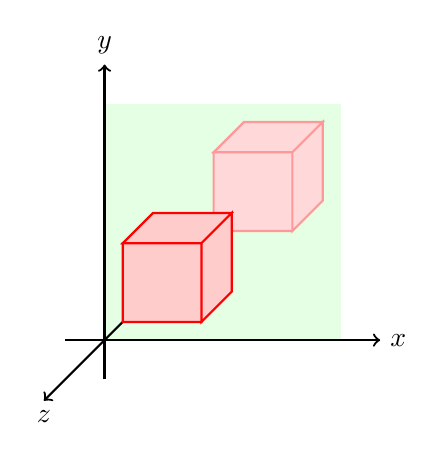
\begin{tikzpicture}


\filldraw [draw=none,fill=green!10!white]
  (0,0) -- (0,3) -- (3,3) -- (3,0) -- cycle;

\draw [->, thick] (0,0,-3) -- (0,0,2) node [below] {$z$};
\draw [->, thick] (0,-0.5,0) -- (0,3.5,0) node [above] {$y$};
\draw [->, thick] (-0.5,0,0) -- (3.5,0,0) node [right] {$x$};

\coordinate (A) at (2,2,2);
\coordinate (B) at (2,2,-1);
\filldraw [thick,draw=red!40,fill=red!15!white] 
  (B) -- ++(0,-1,0) -- ++(-1,0,0) -- ++(0,1,0) -- cycle
  (B) -- ++(0,-1,0) -- ++(0,0,-1) -- ++(0,1,0) -- cycle
  (B) -- ++(-1,0,0) -- ++(0,0,-1) -- ++(1,0,0) -- cycle;
% płaszczyzna symetrii, osie x i y, druga kostka

\filldraw [thick, draw=red,fill=red!20!white] 
  (A) -- ++(0,-1,0) -- ++(-1,0,0) -- ++(0,1,0) -- cycle
  (A) -- ++(0,-1,0) -- ++(0,0,-1) -- ++(0,1,0) -- cycle
  (A) -- ++(-1,0,0) -- ++(0,0,-1) -- ++(1,0,0) -- cycle;




\end{tikzpicture}


\end{document}
